
In dieser Sequenz werden zwei zentrale Aufrufe von \gls{snort} im \gls{praeprozessor} \gls{sppname} dargestellt. Zum einen im oberen Teil die Initialisierung des \gls{praeprozessor}s durch einen Init-Aufruf, sowie der \gls{praeprozessor}-interne Aufbau des DissectorRegisters. Dieser Registrierungsvorgang wurde im Diagramm aus Platzgründen eingespart. Darin wird jeder als C-Datei vorhandene Dissector instanziiert und bei dem DissectorRegister: TopLevelRegister registriert. Dieser Vorgang legt die Grundlage für den Dissector-Baum-Ablauf, welcher exemplarisch als zweiter unterer Teil des Sequenzdiagramms modelliert wurde. Für jedes empfangene Paket ruft \gls{snort} die detectProfinetPackets-Methode in \gls{sppname} auf und übergibt eine Paketpointer. Basierend auf dem Ethertype wählt der TopLevelRegister den ersten Dissector, den für ProfiNet-RealTimes (0x8892 Ethertype) aus und übergibt den Paketpointer. \gls{sppname} ruft in diesem Dissector die dissect-Methode auf, welche basierend auf gefundenen Informationen, sich einen passenden seiner Subdissector, hier den RT1Dissector, aussucht und in diesem die dissect-Methode aufruft. Dieser rekursive Schritt wird solange wiederholt, bis kein Subdissector mehr vorhanden ist oder das Ende des \gls{paket}s gefunden wurde.
Nach der Rückkehr der Methoden wird der fertige ProtocolTree benutzt und ausgelesen, um ein neues \gls{truffle} zu erstellen. Dieses selbstdefinierte \gls{truffle} wird dann mit dem Sender-Interface in Richtung \gls{programname} per \gls{ipc} verschickt.

\begin{figure}[H]
  \centering
  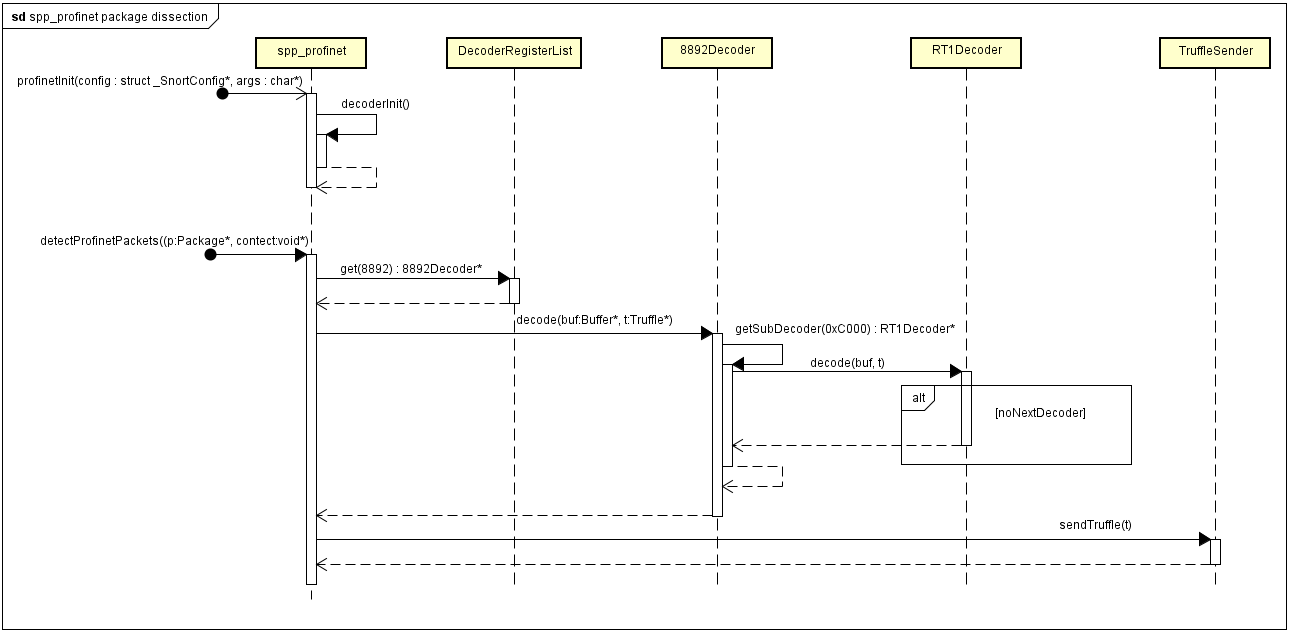
\includegraphics[width=\textwidth]{../diagramimages/spp-profinet-package-dissection.png}
  \caption[Sequenzdiagramm \gls{sppname} package dissection]{Sequenzdiagramm \gls{sppname} package dissection}
  \label{fig:spp_sqd}
\end{figure} 